\section{1174731 - Ainul Filiani}
\subsection{Soal Teori}
\begin{enumerate}

	\item Jelaskan kenapa kata-kata harus di lakukan vektorisasi. dilengkapi dengan ilustrasi atau gambar.
	\hfill\break
	Karena untuk mengetahui persentase kata yang sering muncul di setiap kalimat, yang berguna untuk menentukan kata kunci, dan untuk memberikan kemudahan bagi setiap mesin untuk memfasilitasi kata-kata yang terkait tetapi tidak sama. Selain itu, kata tersebut untuk membaca setiap kata dengan mengubah kata menjadi angka atau identitas itu sendiri. Untuk ilustrasi, lihat gambar berikut: 

	\begin{figure}[H]
	\centering
		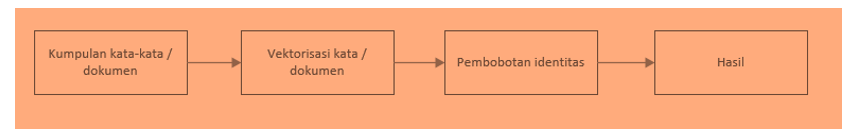
\includegraphics[width=4cm]{figures/1174073/tugas5/materi/teori1.PNG}
		\caption{Teori 1}
	\end{figure}

	\item Jelaskan mengapa dimensi dari vektor dataset google bisa sampai 300. dilengkapi dengan ilustrasi atau gambar.

	\hfill\break
	Karena setiap objek memiliki identitas khusus, misalnya sederhana. Dalam dataset Google ini memiliki 3 objek, kucing, anjing, dan ember yang disetujui. Kemudian dari masing-masing objek dibandingkan dataset antara kucing dan anjing kemudian kucing dan ember. Hasil yang diperoleh untuk kucing dan anjing sekitar 75\% sedangkan untuk kucing dan ember yang memiliki persentase 15\%. Untuk lebih lengkapnya bisa dilihat pada gambar berikut : 

	\begin{figure}[H]
	\centering
		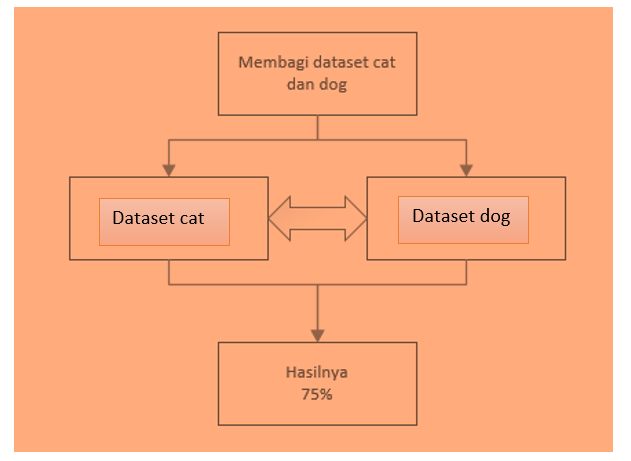
\includegraphics[width=4cm]{figures/1174073/tugas5/materi/teori2.PNG}
		\caption{Teori 2}
	\end{figure}
	
	\item Jelaskan konsep vektorisasi untuk kata.dilengkapi dengan ilustrasi atau gambar.
	\hfill\break
	Konsep untuk vektorisasi kata sama dengan masukan atau input pada kata-kata di mesin pencari. Maka anggaplah itu akan dikeluarkan sebagai saran tentang kata tersebut. Jadi kata data diperoleh dari hasil yang diolah dalam kalimat sebelumnya yang telah diproses. Contoh sederhana dalam kalimat berikut (Silakan berlangganan saluran saya, terima kasih teman), dalam kalimat itu terkait dengan kalimat saluran, kata akan dibuat data pelatihan untuk mesin. Jadi kita kompilasi kata channel, maka mesin akan menampilkan hubungannya dengan kata tersebut. Contoh ilustrasi sederhananya seperti berikut :

	\begin{figure}[H]
	\centering
		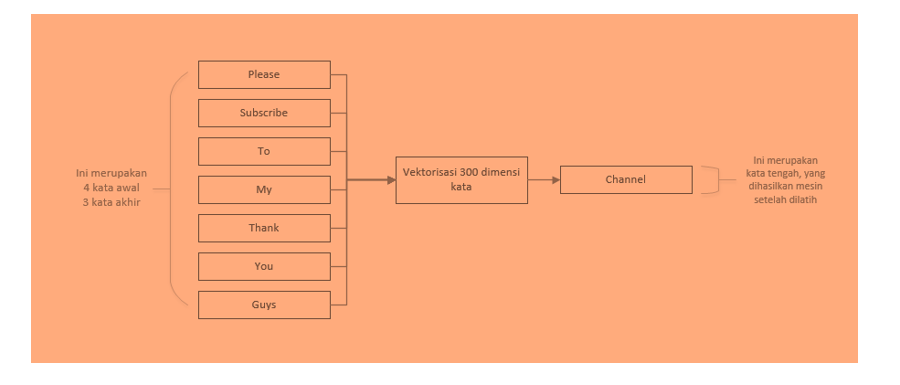
\includegraphics[width=4cm]{figures/1174073/tugas5/materi/teori3.PNG}
		\caption{Teori 3}
	\end{figure}

	\item Jelaskan konsep vektorisasi untuk dokumen.dilengkapi dengan ilustrasi atau gambar.
	\hfill\break
	Sama halnya dengan vektorisasi kata, yang membedakan hanya pada proses awalnya. Untuk vektorisasi dokumen ini, mesin akan membaca semua kalimat yang terdapat pada dokumen tersebut, lalu kalimat yang terdapat pada dokumen akan di pecah menjadi kata-kata. Perhatikan gambar berikut : 

	\begin{figure}[H]
	\centering
		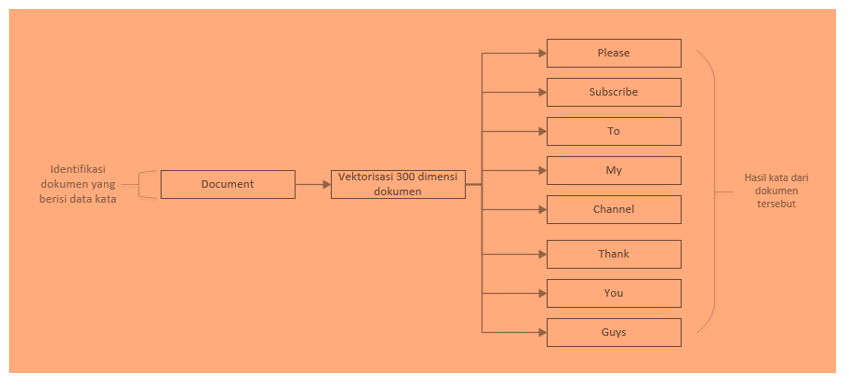
\includegraphics[width=4cm]{figures/1174073/tugas5/materi/teori4.PNG}
		\caption{Teori 4}
	\end{figure}

	\item Jelaskan apa mean dan standar deviasi,dilengkapi dengan ilustrasi atau gambar.
	\hfill\break
	Mean adalah nilai rata-rata. Untuk mendapatkan makna ini, kita hanya perlu menambahkan data yang tersedia dan kemudian membaginya dengan jumlah data. Sedangkan standar deviasi adalah nilai statistik yang digunakan untuk menentukan bagaimana data didistribusikan dalam sampel, dan menentukan titik data individu dengan nilai rata-rata nilai sampel. Rumusnya ialah sebagai berikut :

	\begin{figure}[H]
	\centering
		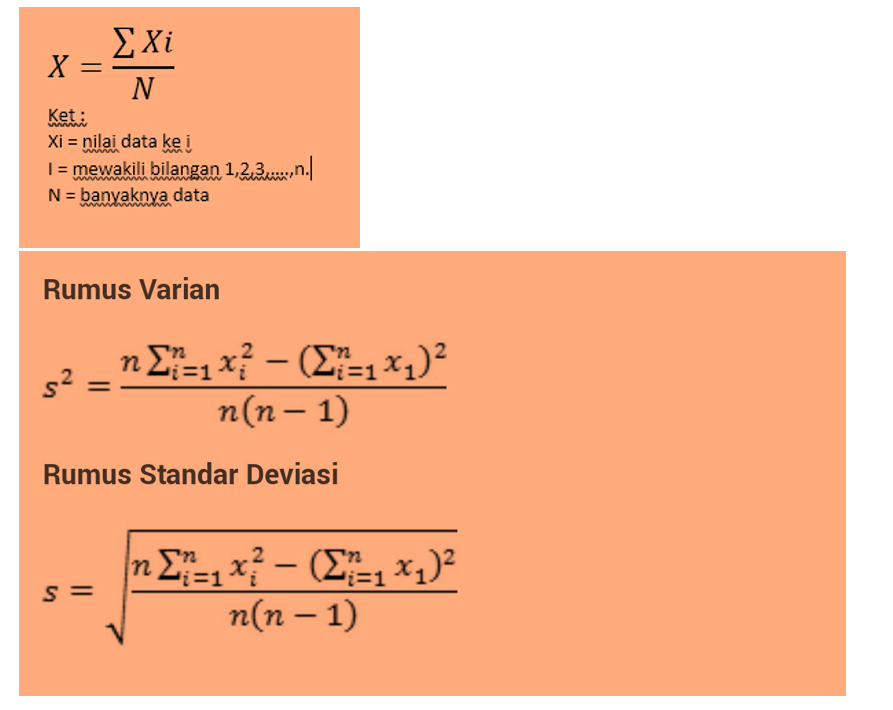
\includegraphics[width=4cm]{figures/1174073/tugas5/materi/teori5.PNG}
		\caption{Teori 5}
	\end{figure}

	\item Jelaskan apa itu skip-gram,dilengkapi dengan ilustrasi atau gambar.
	\hfill\break
	Skip-gram sama halnya dengan vektorisasi kata, namun untuk skip-gram ia dibalik prosesnya. Yang sebelumnya dari kalimat lalu di olah untuk menemukan salah satu kata, kali ini dari keyword tersebut akan diolah menjadi suatu kalimat yang memiliki keterkaitannya dengan keyword tersebut. Contoh sederhananya seperti gambar berikut : 

	\begin{itemize}
			\item Hiyaaa
			\item Ada yang
			\item Copas nih
		\end{itemize}

	\begin{figure}[H]
	\centering
		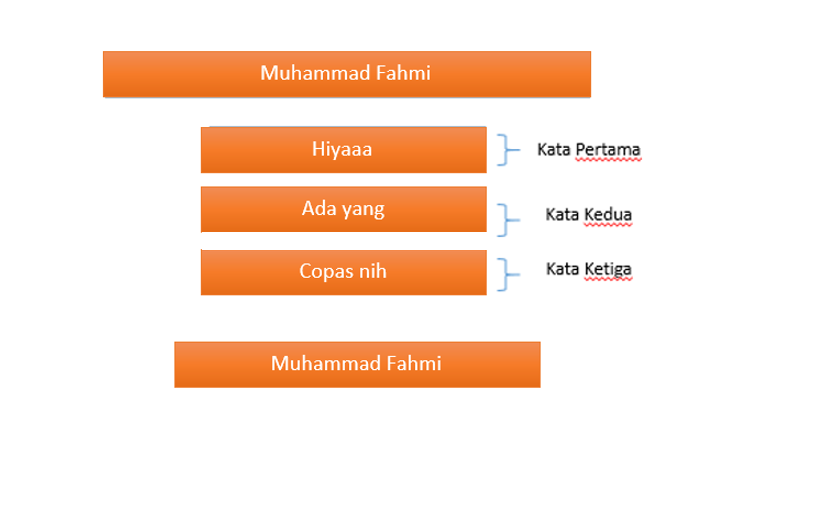
\includegraphics[width=4cm]{figures/1174073/tugas5/materi/teori6.PNG}
		\caption{Teori 6}
	\end{figure}
\end{enumerate}


\subsection{Praktek Program}
\begin{enumerate}
	\item Soal 1
	\hfill\break
	\lstinputlisting[firstline=7, lastline=11]{src/1174073/tugas5/tugas5.py}
	Kode di atas digunakan untuk import library gensim. Gensim itu sendiri berguna untuk melakukan pemodelan dengan dataset atau topik yang telah ditentukan. Untuk keluaran 100 logging itu library opsional karena logging hanya untuk menampilkan berupa log untuk setiap code yang dijalankan. Dan keluaran 101 itu hasil load data dari file vektor google itu, disini saya menggunakan limit karena kondisi laptop yang tidak mempuni untuk melakukan running data sebesar 3 juta file, jadi saya batasi hanya melakukan running 500 ribu data saja, hasilnya ialah sebagai berikut : 
	\begin{figure}[H]
	\centering
		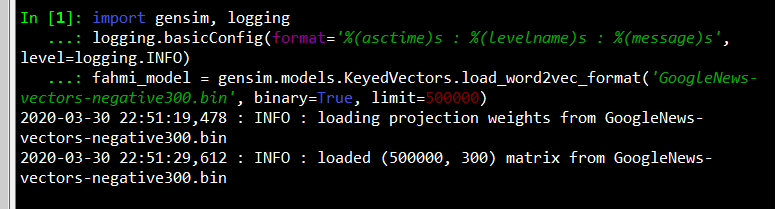
\includegraphics[width=4cm]{figures/1174073/tugas5/materi/hasil1_1.PNG}
		\caption{Hasil Soal 1.}
	\end{figure}

	\hfill\break
	\lstinputlisting[firstline=13, lastline=14]{src/1174073/tugas5/tugas5.py}
	ini untuk menampilkan data hasil vektorisasi data dari kata love, hasilnya ialah sebagai berikut : 
	\begin{figure}[H]
	\centering
		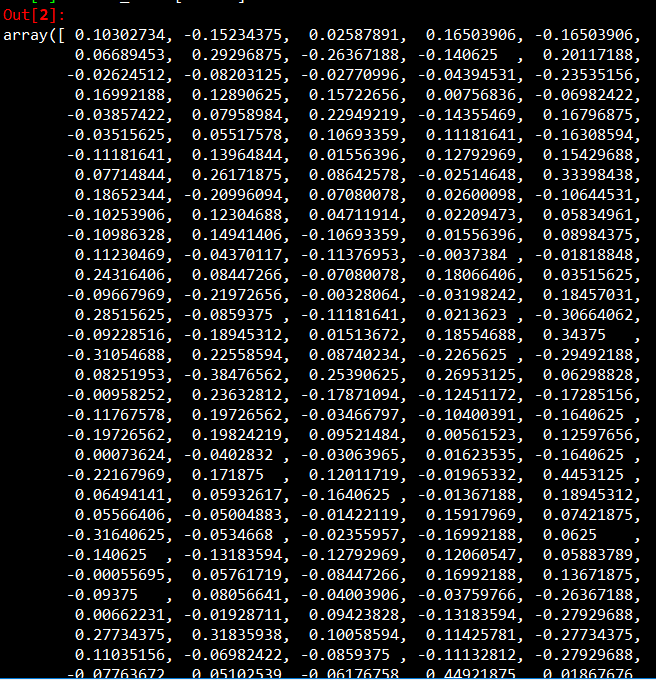
\includegraphics[width=4cm]{figures/1174073/tugas5/materi/hasil1_2.PNG}
	\end{figure}

	\hfill\break
	\lstinputlisting[firstline=15, lastline=16]{src/1174073/tugas5/tugas5.py}
	ini untuk menampilkan data hasil vektorisasi data dari kata faith, hasilnya ialah sebagai berikut : 
	\begin{figure}[H]
	\centering
		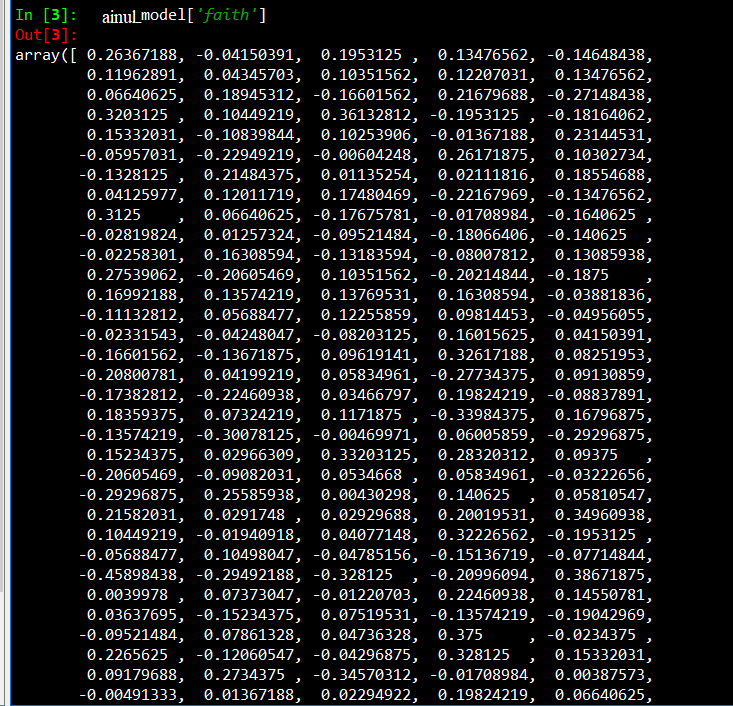
\includegraphics[width=4cm]{figures/1174073/tugas5/materi/hasil1_3.PNG}
	\end{figure}

	\hfill\break
	\lstinputlisting[firstline=17, lastline=18]{src/1174073/tugas5/tugas5.py}
	ini untuk menampilkan data hasil vektorisasi data dari kata fall, hasilnya ialah sebagai berikut : 
	\begin{figure}[H]
	\centering
		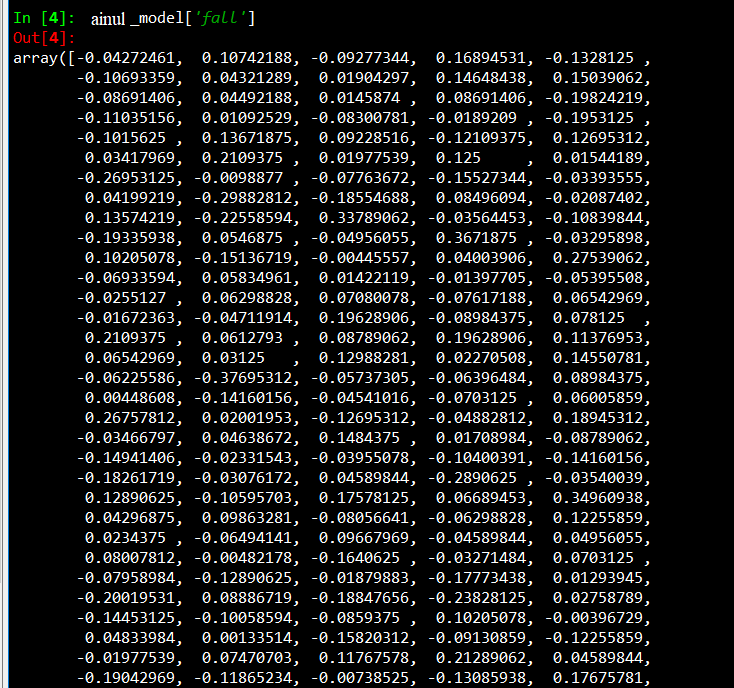
\includegraphics[width=4cm]{figures/1174073/tugas5/materi/hasil1_4.PNG}
	\end{figure}

	\hfill\break
	\lstinputlisting[firstline=19, lastline=20]{src/1174073/tugas5/tugas5.py}
	ini untuk menampilkan data hasil vektorisasi data dari kata sick, hasilnya ialah sebagai berikut : 
	\begin{figure}[H]
	\centering
		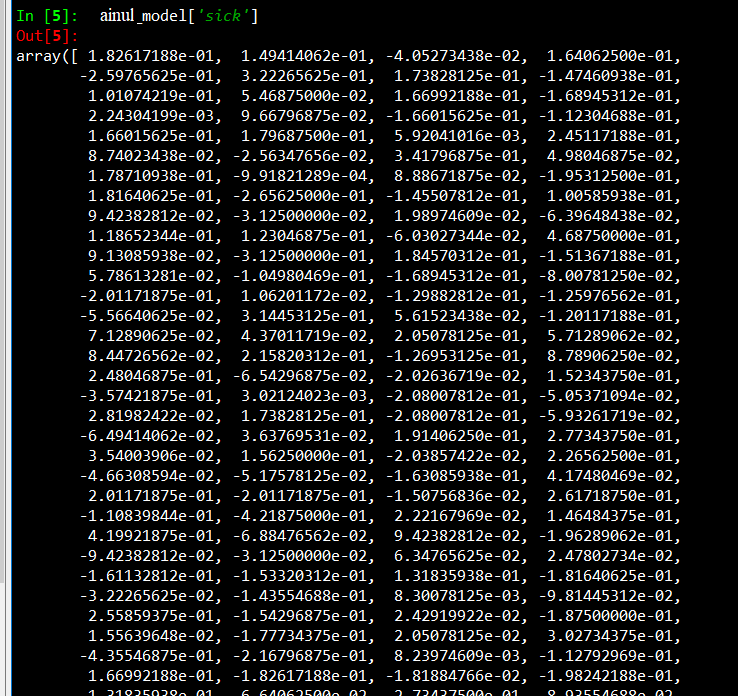
\includegraphics[width=4cm]{figures/1174073/tugas5/materi/hasil1_5.PNG}
	\end{figure}

	\hfill\break
	\lstinputlisting[firstline=21, lastline=22]{src/1174073/tugas5/tugas5.py}
	ini untuk menampilkan data hasil vektorisasi data dari kata clear, hasilnya ialah sebagai berikut : 
	\begin{figure}[H]
	\centering
		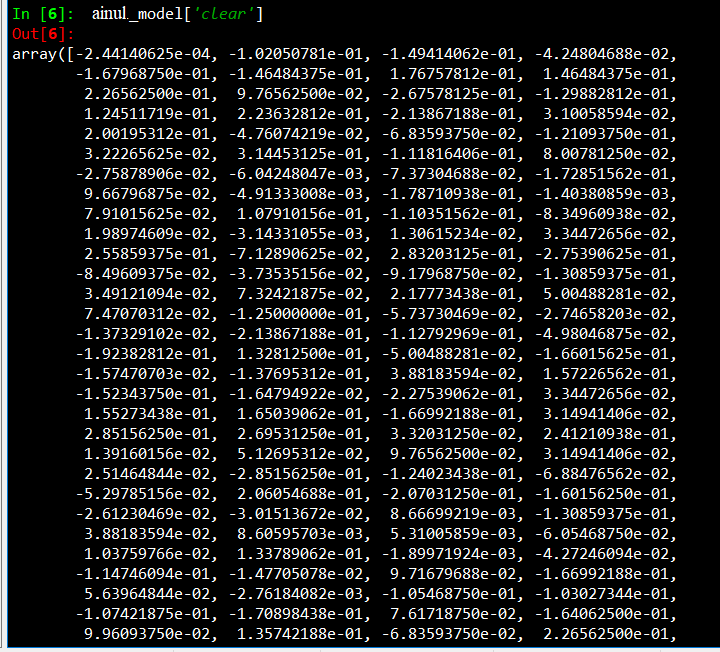
\includegraphics[width=4cm]{figures/1174073/tugas5/materi/hasil1_6.PNG}
	\end{figure}

	\hfill\break
	\lstinputlisting[firstline=23, lastline=24]{src/1174073/tugas5/tugas5.py}
	ini untuk menampilkan data hasil vektorisasi data dari kata shine, hasilnya ialah sebagai berikut : 
	\begin{figure}[H]
	\centering
		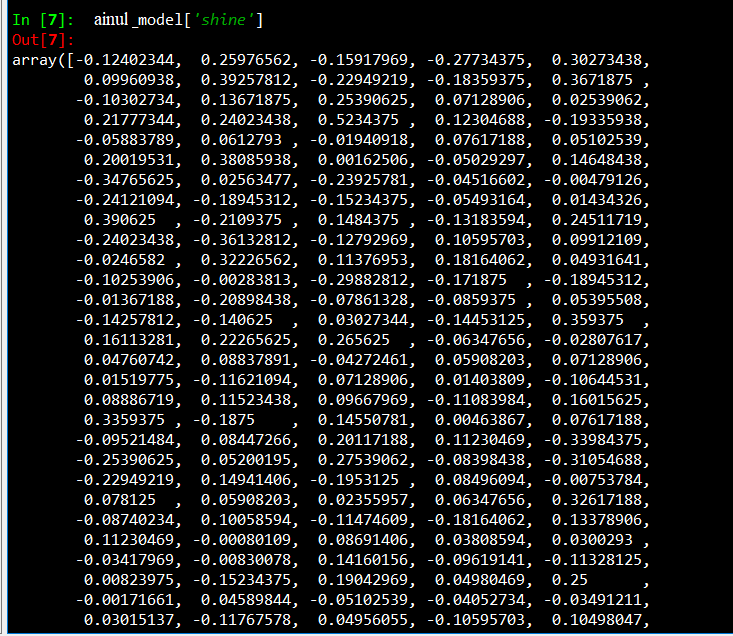
\includegraphics[width=4cm]{figures/1174073/tugas5/materi/hasil1_7.PNG}
	\end{figure}

	\hfill\break
	\lstinputlisting[firstline=25, lastline=26]{src/1174073/tugas5/tugas5.py}
	ini untuk menampilkan data hasil vektorisasi data dari kata bag, hasilnya ialah sebagai berikut : 
	\begin{figure}[H]
	\centering
		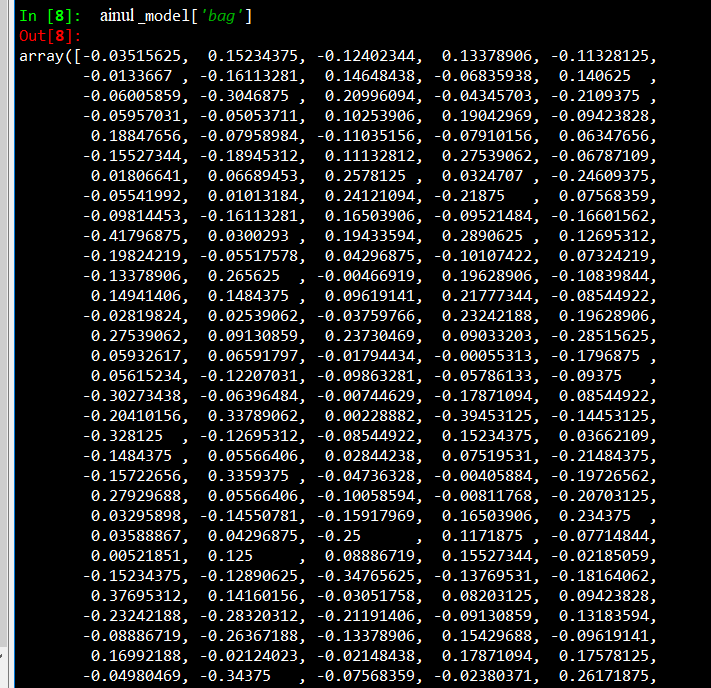
\includegraphics[width=4cm]{figures/1174073/tugas5/materi/hasil1_8.PNG}
	\end{figure}

	\hfill\break
	\lstinputlisting[firstline=27, lastline=28]{src/1174073/tugas5/tugas5.py}
	ini untuk menampilkan data hasil vektorisasi data dari kata car, hasilnya ialah sebagai berikut : 
	\begin{figure}[H]
	\centering
		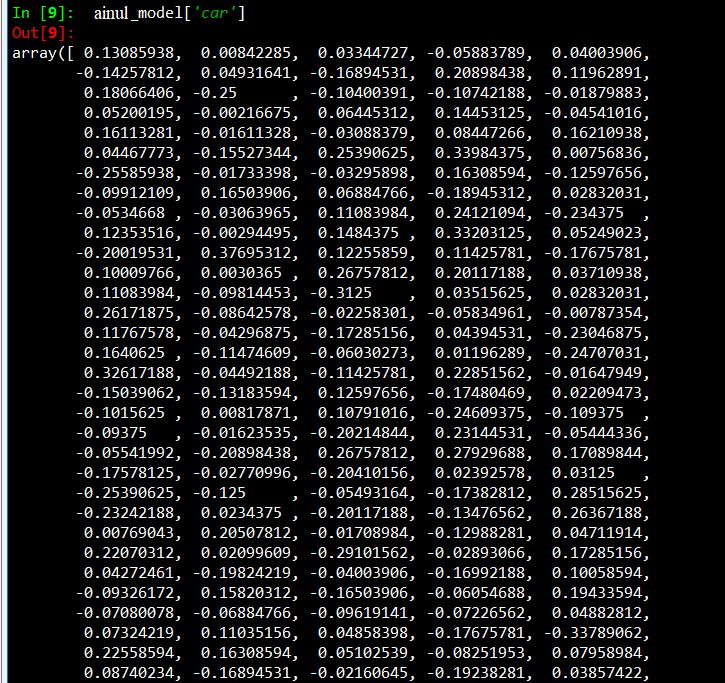
\includegraphics[width=4cm]{figures/1174073/tugas5/materi/hasil1_9.PNG}
	\end{figure}

	\hfill\break
	\lstinputlisting[firstline=29, lastline=30]{src/1174073/tugas5/tugas5.py}
	ini untuk menampilkan data hasil vektorisasi data dari kata wash, hasilnya ialah sebagai berikut : 
	\begin{figure}[H]
	\centering
		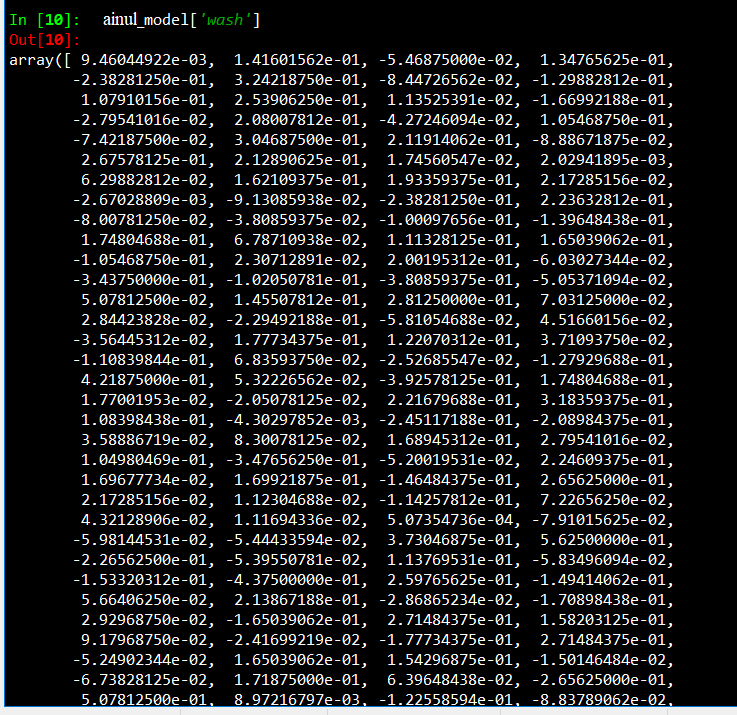
\includegraphics[width=4cm]{figures/1174073/tugas5/materi/hasil1_10.PNG}
	\end{figure}

	\hfill\break
	\lstinputlisting[firstline=31, lastline=32]{src/1174073/tugas5/tugas5.py}
	ini untuk menampilkan data hasil vektorisasi data dari kata motor, hasilnya ialah sebagai berikut : 
	\begin{figure}[H]
	\centering
		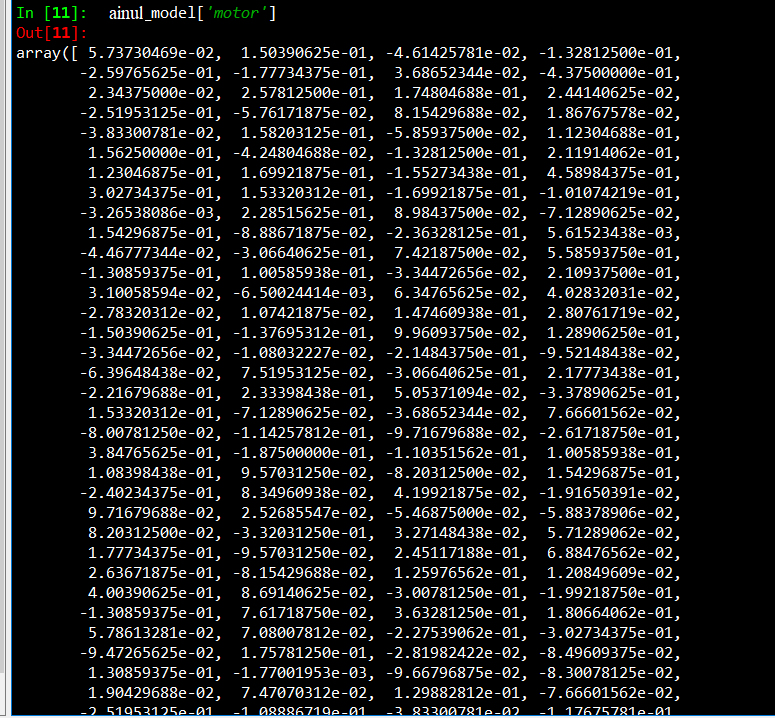
\includegraphics[width=4cm]{figures/1174073/tugas5/materi/hasil1_11.PNG}
	\end{figure}

	\hfill\break
	\lstinputlisting[firstline=33, lastline=34]{src/1174073/tugas5/tugas5.py}
	ini untuk menampilkan data hasil vektorisasi data dari kata cycle, hasilnya ialah sebagai berikut : 
	\begin{figure}[H]
	\centering
		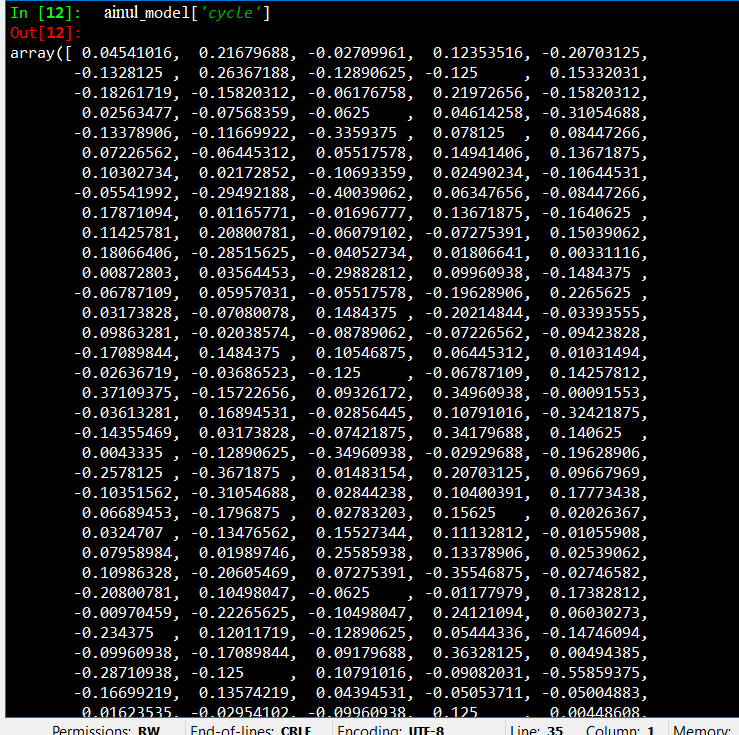
\includegraphics[width=4cm]{figures/1174073/tugas5/materi/hasil1_12.PNG}
	\end{figure}

	\hfill\break
	\lstinputlisting[firstline=35, lastline=36]{src/1174073/tugas5/tugas5.py}
	Ini merupakan persentase dari perbandingan kata wash dan clear, persentase yang di dapat ialah 9 \% Hasil tersebut tidak terlalu baik, ialah sebagai berikut : 
	\begin{figure}[H]
	\centering
		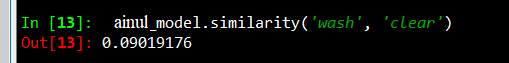
\includegraphics[width=4cm]{figures/1174073/tugas5/materi/hasil1_13.PNG}
	\end{figure}

	\hfill\break
	\lstinputlisting[firstline=37, lastline=38]{src/1174073/tugas5/tugas5.py}
	Ini merupakan persentase dari perbandingan kata bag dan love, persentase yang di dapat ialah 7 \% Hasil tersebut tidak terlalu baik, ialah sebagai berikut 
	\begin{figure}[H]
	\centering
		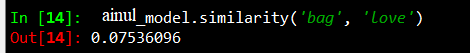
\includegraphics[width=4cm]{figures/1174073/tugas5/materi/hasil1_14.PNG}
	\end{figure}

	\hfill\break
	\lstinputlisting[firstline=39, lastline=40]{src/1174073/tugas5/tugas5.py}
	Ini merupakan persentase dari perbandingan kata motor dan car, persentase yang di dapat ialah 48 \% Hasil tersebut cukup baik karena mesin dapat membedakan antara motor dan car, ialah sebagai berikut 
	\begin{figure}[H]
	\centering
		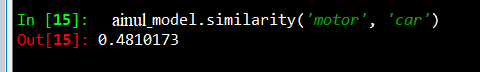
\includegraphics[width=4cm]{figures/1174073/tugas5/materi/hasil1_15.PNG}
	\end{figure}

	\hfill\break
	\lstinputlisting[firstline=41, lastline=42]{src/1174073/tugas5/tugas5.py}
	Ini merupakan persentase dari perbandingan kata sick dan faith, persentase yang di dapat ialah 12 \% Hasil tersebut lumayan dibawah cukup, ialah sebagai berikut 
	\begin{figure}[H]
	\centering
		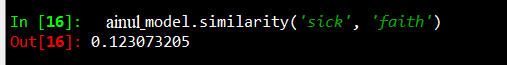
\includegraphics[width=4cm]{figures/1174073/tugas5/materi/hasil1_16.PNG}
	\end{figure}

	\hfill\break
	\lstinputlisting[firstline=43, lastline=44]{src/1174073/tugas5/tugas5.py}
	Ini merupakan persentase dari perbandingan kata cycle dan shine, persentase yang di dapat ialah 9 \% Hasil tersebut buruk karena begitu sedikit persentase yang didapat, ialah sebagai berikut 
	\begin{figure}[H]
	\centering
		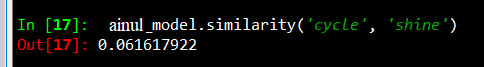
\includegraphics[width=4cm]{figures/1174073/tugas5/materi/hasil1_17.PNG}
	\end{figure}


	\item Soal 2
	\hfill\break
	\lstinputlisting[firstline=46, lastline=54]{src/1174073/tugas5/tugas5.py}
	Kode tersebut berguna untuk membuat string memakai import re, dengan memakai test\_string sebagai string, dan membuat print untuk menambahkan kalimat sebelum test\_string, hasilnya sebagai berikut :
	\begin{figure}[H]
	\centering
		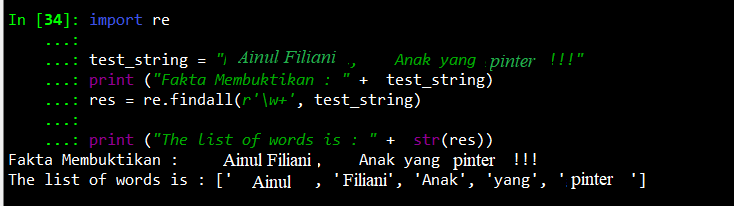
\includegraphics[width=4cm]{figures/1174073/tugas5/materi/hasil2_1.PNG}
		\caption{Hasil Soal 2}
	\end{figure}

	\hfill\break
	\lstinputlisting[firstline=56, lastline=70]{src/1174073/tugas5/tugas5.py}
	Kode tersebut berguna untuk membuat string memakai import random, dengan memakai sent\_matrix untuk membuat string, dan result sebagai print random yang akan diacak, hasilnya bisa berubah-ubah, sebagai berikut :
	\begin{figure}[H]
	\centering
		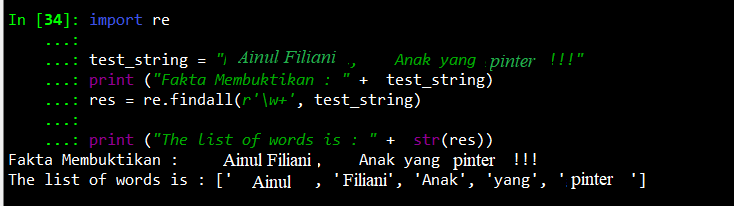
\includegraphics[width=4cm]{figures/1174073/tugas5/materi/hasil2_1.PNG}
		\caption{Hasil Soal 2}
	\end{figure}
	
	\item Soal 3
	\hfill\break
	\lstinputlisting[firstline=72, lastline=99]{src/1174073/tugas5/tugas5.py}
	Fungsi dari library gensim untuk pemodelan topik tanpa pengawasan dan pemrosesan bahasa alami, atau bisa kita sebut dengan unsupervised. Fungsi dari doc2vec itu sendiri ialah untuk membandingkan bobot data yang terdapat pada dokumen yang lainnya, apakah kata-kata didalamnya ada yang sama atau tidak. Lalu untuk tagged document itu memasukan kata-kata pada setiap dokumennya untuk di vektorisasi, dan model untuk membuat model dan save file model. Hasilnya adalah sebagai berikut :
	\begin{figure}[H]
	\centering
		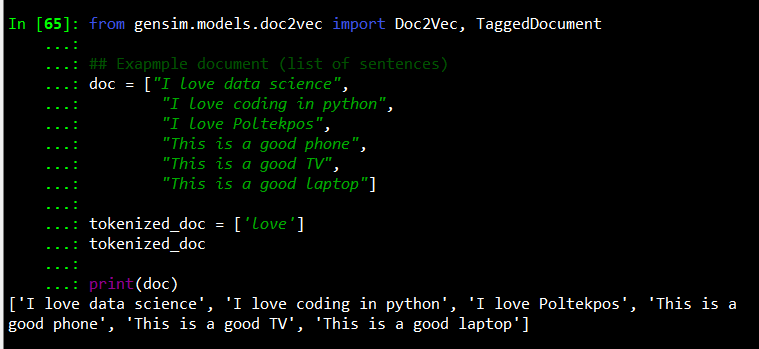
\includegraphics[width=4cm]{figures/1174073/tugas5/materi/hasil3_1.PNG}
		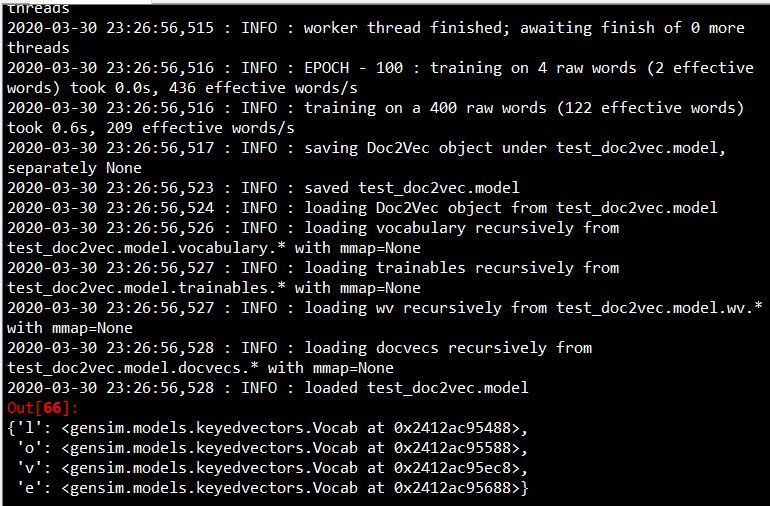
\includegraphics[width=4cm]{figures/1174073/tugas5/materi/hasil3_2.PNG}
		
\includegraphics[width=4cm]{figures/1174073/tugas5/materi/hasil3_3.PNG}
		\caption{Hasil Soal 3}
	\end{figure}

	\item Soal 4
	\hfill\break
	\lstinputlisting[firstline=102, lastline=114]{src/1174073/tugas5/tugas5.py}
	Disini kita memakai dataset dari aclImdb. Untuk menambahkan data training kita melakukan import library os, library os itu sendiri berfungsi untuk melakukan interaksi antara python dengan os laptop kita masing-masing, setelah itu kita buat variable unsup sentences. Selanjutnya pilih direktori tempat data kita disimpan. Selanjutnya itu untuk menyortir data yang terdapat pada folder aclImdb dan membaca file tersebut dengan ektensi .txt. Hasil dari code pertama tersebut ialah terdapatnya data hasil running dari folder aclImdb. Hasilnya adalah sebagai berikut :
	\begin{figure}[H]
	\centering
		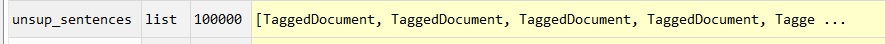
\includegraphics[width=4cm]{figures/1174073/tugas5/materi/hasil4_1.PNG}
		\caption{Hasil Soal 4.}
	\end{figure}

	\item Soal 5
	\hfill\break
	\lstinputlisting[firstline=117, lastline=123]{src/1174073/tugas5/tugas5.py}
	Untuk bagian pengacakan data itu berguna untuk mengacak data supaya pada saat data di running bisa berjalan lebih baik dan hasil presentase akhirnya bisa lebih baik. Sedangkan untuk pembersihan data untuk memberikan ruang bagi ram laptop kita setelah melakukan running data sebanyak 3 juta lebih, agar lebih ringan saat proses selanjutnya. Hasilnya adalah sebagai berikut :
	\begin{figure}[H]
	\centering
		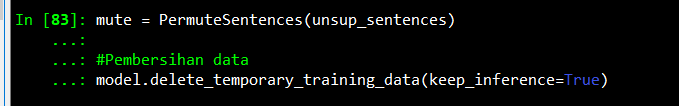
\includegraphics[width=4cm]{figures/1174073/tugas5/materi/hasil5_1.PNG}
		\caption{Hasil Soal 5.}
	\end{figure}

	\item Soal 6
	\hfill\break
	\lstinputlisting[firstline=126, lastline=132]{src/1174073/tugas5/tugas5.py}
	Save data ini berfungsi untuk menyimpan file hasil dari proses pelatihan data sebelumnya, model tersebut dilakukan penyimpanan untuk memberikan keringanan pada ram agar saat kita akan melakukan pelatihan lagi, model tersebut tinggal di load saja tanpa harus melakukan pelatihan dari awal dan bisa menghemat waktu. Sedangkan untuk delete temporary training data ini berguna untuk menghapus data latihan yang sebelumnya sudah dilakukan dan disimpan, bertujuan untuk memberikan keringanan pada ram. Karena setelah melakukan proses pelatihan ram biasanya jadi tercekik sampai laptop jadi lag. Itulah fungsi dari delete temporary training data. Hasilnya adalah sebagai berikut :
	\begin{figure}[H]
	\centering
		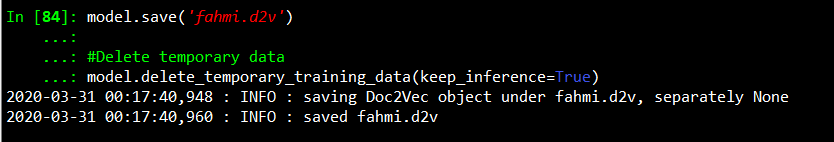
\includegraphics[width=4cm]{figures/1174073/tugas5/materi/hasil6_1.PNG}
		\caption{Hasil Soal 6.}
	\end{figure}

	\item Soal 7
	\hfill\break
	\lstinputlisting[firstline=134, lastline=136]{src/1174073/tugas5/tugas5.py}
	Infer vector itu sendiri berguna untuk membandingkan kata yang tercantum dengan vektor yang mana pada dokumen yang sudah di load pada step sebelumnya. Selain itu infer vector juga untuk menghitung atau mengkalkulasikan vektor dari kata yang dicantumkan dari model yang telah kita buat. Alangkah baiknya kata yang dicantumkan itu lebih panjang lagi agar hasilnya bisa lebih baik lagi. Hasilnya adalah sebagai berikut :
	\begin{figure}[H]
	\centering
		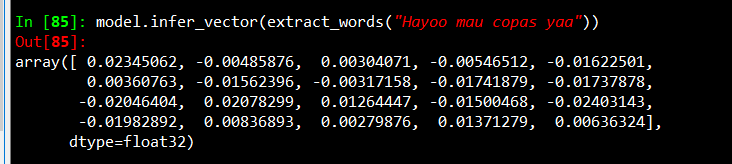
\includegraphics[width=4cm]{figures/1174073/tugas5/materi/hasil7_1.PNG}
		\caption{Hasil Soal 7.}
	\end{figure}

	\item Soal 8
	\hfill\break
	\lstinputlisting[firstline=138, lastline=143]{src/1174073/tugas5/tugas5.py}
	Cosine similarity ini berfungsi untuk membandingkan vektorisasi data diantara kedua kata yang di inputkan, jika hasil presentase dari kedua kata tersebut lebih dari 50\% itu memiliki kemungkinan kata tersebut terdapat dalam 1 file. Namun jika kurang dari 50\% itu kemungkinan kata tersebut tidak terdapat dalam 1 file. Hasil yang didapatkan pada code tersebut hanya 0.8\% itu dikarenakan kata pertama dan kedua tidak memiliki kesamaan vektorisasi dan tidak terdapat pada salah satu dokumen. Hasilnya adalah sebagai berikut :
	\begin{figure}[H]
	\centering
		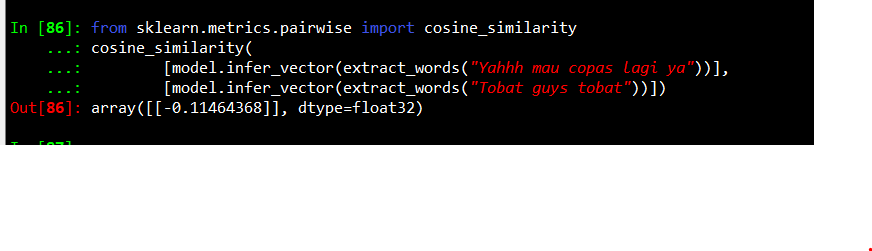
\includegraphics[width=4cm]{figures/1174073/tugas5/materi/hasil8_1.PNG}
		\caption{Hasil Soal 8.}
	\end{figure}

	\item Soal 9
	\hfill\break
	\lstinputlisting[firstline=145, lastline=153]{src/1174073/tugas5/tugas5.py}
	Code tersebut akan melakukan perhitungan presentase dengan menggunakan cross validation dengan metode kneighborsClassifier. Memakai dataset iris, hasilnya adalah sebagai berikut :
	\begin{figure}[H]	\centering
		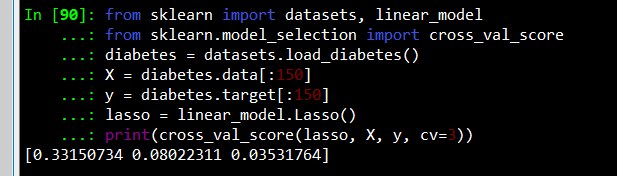
\includegraphics[width=4cm]{figures/1174073/tugas5/materi/hasil9_1.PNG}
		\caption{Hasil Soal 9.}
	\end{figure}
\end{enumerate}

\subsection{Penanganan Error}
\begin{enumerate}
	\item ScreenShoot Error
	\begin{figure}[H]
		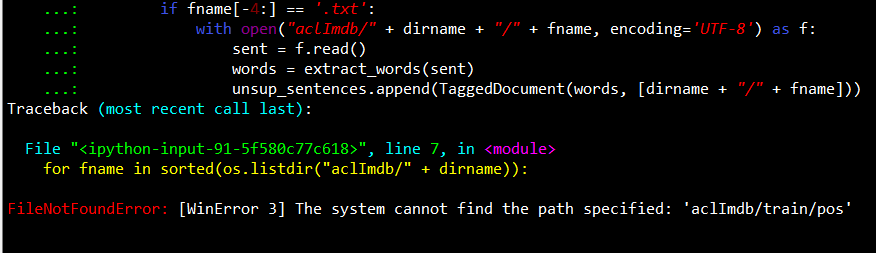
\includegraphics[width=4cm]{figures/1174073/tugas5/error/1.PNG}
		\centering
		\caption{FileNotFoundError}
	\end{figure}
	\item Cara Penanganan Error
	\begin{itemize}
		\item FileNotFoundError
		\hfill\break
		Error terdapat pada dataset yang tidak terbaca, dengan ini saya mendownload dataset dari aclImdb, dan masalah error telah selesai.
	\end{itemize}
\end{enumerate}

\subsection{Bukti Tidak Plagiat}
\begin{figure}[H]
\centering
	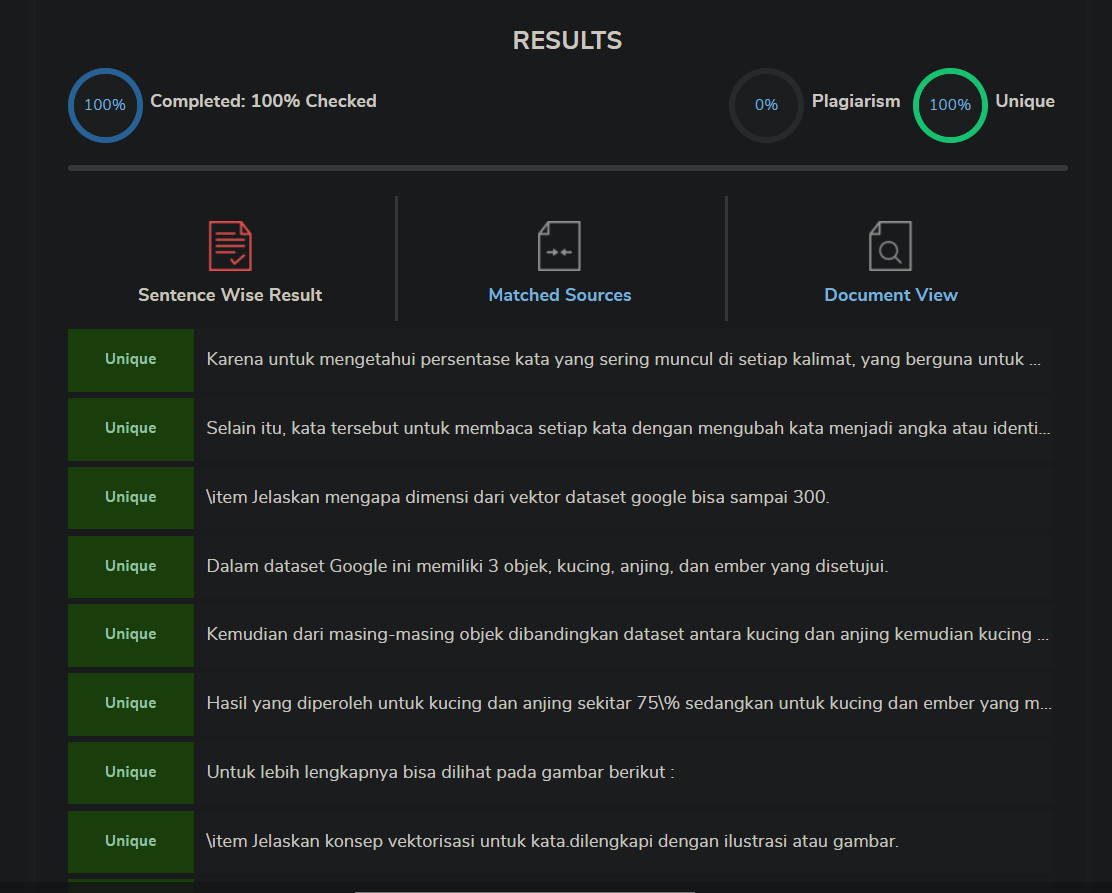
\includegraphics[width=4cm]{figures/1174073/tugas5/buktiplagiat/1.PNG}
	\caption{Bukti Tidak Melakukan Plagiat Chapter 5}
\end{figure}

